% Presentatie Project 7 (tussentijds)
\documentclass{beamer}

\mode<presentation>

\usepackage[dutch]{babel}
%\usepackage{beamerthemesplit}
\usetheme{Berlin}
\useinnertheme{rounded}
\usecolortheme{rose}
\setbeamertemplate{navigation symbols}{} 

\title{Project voortgang}
\author{
  Sebastiaan Polderman (0820738)
  \and
  Paul Sohier (0806122)}
\date{\today}

\begin{document}

\frame{
  \titlepage
} 

\frame{
  \frametitle{Inhoud}
  \tableofcontents
}

\section{Introductie}
 \frame{
   \frametitle{Wie zijn wij}
   \begin{itemize}
    \item<1-> Sebastiaan Polderman (0820738)
    \item<2-> Paul Sohier (0806122)
   \end{itemize}
}

\section{Onderzoek}
\frame{
  \frametitle{Werking fluffy}
  \begin{itemize}
   %    \item<1-> 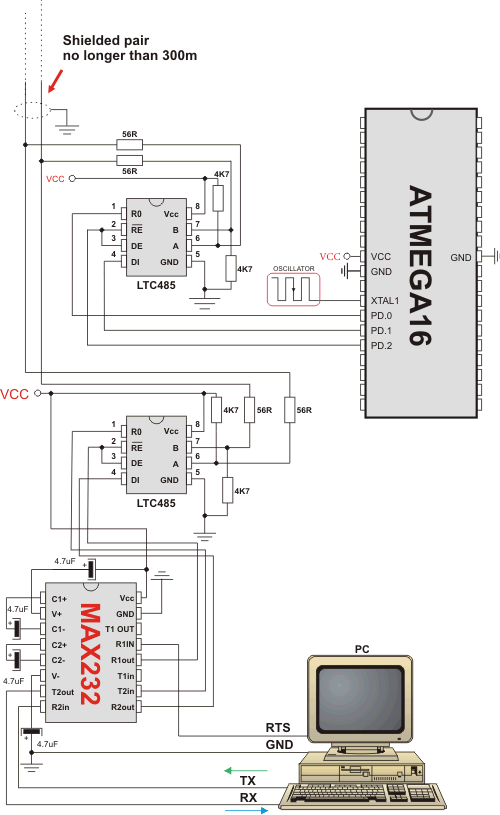
\includegraphics[scale=0.2]{scheme_rs485.pdf}
   \item<1-> Motor gebruik (en nummers)
   \item<2-> Huidige functies
   \item<3-> Algemene werking
   \item<4-> Uitzoeken manier om schroeven te bevestigen zodat ze niet losraken. \\ Dit was het grootste probleem bij de huidige fluffy.
  \end{itemize}
}

\frame{
  \frametitle{Voortgang}
  \begin{itemize}
   \item<1-> Begonnen opbouw poten
   \item<2-> Onderzoek algemene opbouw
  \end{itemize}
}

\section{Afsluiting}
\frame{
  \frametitle{Afsluiting}
  
  Zijn er nog vragen?
}

\end{document}
